% This is "sig-alternate.tex" V2.1 April 2013
% This file should be compiled with V2.5 of "sig-alternate.cls" May 2012
%
% This example file demonstrates the use of the 'sig-alternate.cls'
% V2.5 LaTeX2e document class file. It is for those submitting
% articles to ACM Conference Proceedings WHO DO NOT WISH TO
% STRICTLY ADHERE TO THE SIGS (PUBS-BOARD-ENDORSED) STYLE.
% The 'sig-alternate.cls' file will produce a similar-looking,
% albeit, 'tighter' paper resulting in, invariably, fewer pages.
%
% ----------------------------------------------------------------------------------------------------------------
% This .tex file (and associated .cls V2.5) produces:
%       1) The Permission Statement
%       2) The Conference (location) Info information
%       3) The Copyright Line with ACM data
%       4) NO page numbers
%
% as against the acm_proc_article-sp.cls file which
% DOES NOT produce 1) thru' 3) above.
%
% Using 'sig-alternate.cls' you have control, however, from within
% the source .tex file, over both the CopyrightYear
% (defaulted to 200X) and the ACM Copyright Data
% (defaulted to X-XXXXX-XX-X/XX/XX).
% e.g.
% \CopyrightYear{2007} will cause 2007 to appear in the copyright line.
% \crdata{0-12345-67-8/90/12} will cause 0-12345-67-8/90/12 to appear in the copyright line.
%
% ---------------------------------------------------------------------------------------------------------------
% This .tex source is an example which *does* use
% the .bib file (from which the .bbl file % is produced).
% REMEMBER HOWEVER: After having produced the .bbl file,
% and prior to final submission, you *NEED* to 'insert'
% your .bbl file into your source .tex file so as to provide
% ONE 'self-contained' source file.
%
% ================= IF YOU HAVE QUESTIONS =======================
% Questions regarding the SIGS styles, SIGS policies and
% procedures, Conferences etc. should be sent to
% Adrienne Griscti (griscti@acm.org)
%
% Technical questions _only_ to
% Gerald Murray (murray@hq.acm.org)
% ===============================================================
%
% For tracking purposes - this is V2.0 - May 2012
\newcommand{\refalg}[1]{Algorithm~\ref{#1}}
\newcommand{\refsec}[1]{Sect.~\ref{#1}}
\newcommand{\reffig}[1]{Fig.~\ref{#1}}
\newcommand{\refsubfig}[1]{Fig.~\subref{#1}}
\newcommand{\reftab}[1]{Table~\ref{#1}}
\newcommand{\refeqn}[1]{(\ref{#1})}
\newcommand{\reflst}[1]{Listing~(\ref{#1})}
\newcommand{\bigo}[1]{\mathcal{O}(#1)}

\documentclass{sig-alternate}

\usepackage{subfigure}

\begin{document}

% Copyright
\setcopyright{acmcopyright}
%\setcopyright{acmlicensed}
%\setcopyright{rightsretained}
%\setcopyright{usgov}
%\setcopyright{usgovmixed}
%\setcopyright{cagov}
%\setcopyright{cagovmixed}


% DOI
%\doi{000000} ??????  

% ISBN
%\isbn{000000} ???????

%Conference
\conferenceinfo{EASC '16}{April 26--29, 2016, Stockholm, Sweden}

%\acmPrice{\$15.00}

%
% --- Author Metadata here ---
\conferenceinfo{EASC2016}{'16, Stockholm, Sweden}
%\CopyrightYear{2007} % Allows default copyright year (20XX) to be over-ridden - IF NEED BE.
%\crdata{0-12345-67-8/90/01}  % Allows default copyright data (0-89791-88-6/97/05) to be over-ridden - IF NEED BE.
% --- End of Author Metadata ---

\title{Scaling Behavior of Nek5000}
\subtitle{Subtitle}
%
% You need the command \numberofauthors to handle the 'placement
% and alignment' of the authors beneath the title.
%
% For aesthetic reasons, we recommend 'three authors at a time'
% i.e. three 'name/affiliation blocks' be placed beneath the title.
%
% NOTE: You are NOT restricted in how many 'rows' of
% "name/affiliations" may appear. We just ask that you restrict
% the number of 'columns' to three.
%
% Because of the available 'opening page real-estate'
% we ask you to refrain from putting more than six authors
% (two rows with three columns) beneath the article title.
% More than six makes the first-page appear very cluttered indeed.
%
% Use the \alignauthor commands to handle the names
% and affiliations for an 'aesthetic maximum' of six authors.
% Add names, affiliations, addresses for
% the seventh etc. author(s) as the argument for the
% \additionalauthors command.
% These 'additional authors' will be output/set for you
% without further effort on your part as the last section in
% the body of your article BEFORE References or any Appendices.

\numberofauthors{6} %  in this sample file, there are a *total*
% of EIGHT authors. SIX appear on the 'first-page' (for formatting
% reasons) and the remaining two appear in the \additionalauthors section.
%
\author{
% You can go ahead and credit any number of authors here,
% e.g. one 'row of three' or two rows (consisting of one row of three
% and a second row of one, two or three).
%
% The command \alignauthor (no curly braces needed) should
% precede each author name, affiliation/snail-mail address and
% e-mail address. Additionally, tag each line of
% affiliation/address with \affaddr, and tag the
% e-mail address with \email.
%
% 1st. author
% 1st. author
\alignauthor
Oana Marin\\
       \affaddr{*}\\
       \affaddr{*}\\
       \affaddr{*}\\
       \email{*}
% 2nd. author
\alignauthor
Nicolas Offermans\\
       \affaddr{Linn\'{e} Flow Center}\\
       \affaddr{KTH Mechanics, Royal Institute of Technology}\\
       \affaddr{10044 Stockholm, Sweden}\\
       \email{nof@mech.kth.se}
% 3rd. author
\alignauthor 
Adam Peplinski\\
       \affaddr{*}\\
       \affaddr{*}\\
       \affaddr{*}\\
       \email{*}
\and  % use '\and' if you need 'another row' of author names
% 4th. author
\alignauthor 
Michel Schanen\\
       \affaddr{*}\\
       \affaddr{*}\\
       \affaddr{*}\\
       \email{*}
% 5th. author
\alignauthor 
Philipp Schlatter\\
       \affaddr{*}\\
       \affaddr{*}\\
       \affaddr{*}\\
       \email{*}
% 6th. author
\alignauthor
Jing Gong\\
       \affaddr{PDC-HPC}\\
       \affaddr{KTH, Royal Institute of Technology}\\
       \affaddr{10044 Stockholm, Sweden}\\
       \email{gongjing@kth.se}
}
% There's nothing stopping you putting the seventh, eighth, etc.
% author on the opening page (as the 'third row') but we ask,
% for aesthetic reasons that you place these 'additional authors'
% in the \additional authors block, viz.
%\additionalauthors{Additional authors: John Smith (The Th{\o}rv{\"a}ld Group,
%email: {\texttt{jsmith@affiliation.org}}) and Julius P.~Kumquat
%(The Kumquat Consortium, email: {\texttt{jpkumquat@consortium.net}}).}
\date{21 March 2016}
% Just remember to make sure that the TOTAL number of authors
% is the number that will appear on the first page PLUS the
% number that will appear in the \additionalauthors section.

\maketitle
\begin{abstract}
In this paper, strong scaling and benchmarking of the high-order spectral element solver Nek5000 are performed. The previous extensive benchmarking for Nek5000 was done for terascale computers. This study updates the results to modern computers and assess the ability of the code to run efficiently on the next generation of exascale supercomputers. For several test cases, the main blocks of the code are timed and a sampling tool is use to measure the communication time over a large range of processors. The test cases correspond to a turbulent flow in a straight pipe at four different friction Reynolds numbers $Re_{\tau} = 180$, $360$, $550$ and $1000$. Different architectures are studied, namely IBM Blue Gene/Q, Cray XC40 and Cray XK7 supercomputers. A theoretical model for parallel performance is introduced and compared to the numerical results. We also study the effect of the two coarse grid solvers XXT and AMG on the computational time.
\end{abstract}


% Code generated by the tool at
% http://dl.acm.org/ccs.cfm
%
% I generated what follows quite arbitrarily... Do not hesitate to modify.
% Is it even necessary?
 \begin{CCSXML}
<ccs2012>
<concept>
<concept_id>10010147.10010169.10010170</concept_id>
<concept_desc>Computing methodologies~Parallel algorithms</concept_desc>
<concept_significance>500</concept_significance>
</concept>
<concept>
<concept_id>10010147.10010169.10010170.10010174</concept_id>
<concept_desc>Computing methodologies~Massively parallel algorithms</concept_desc>
<concept_significance>300</concept_significance>
</concept>
<concept>
<concept_id>10003752.10003777.10003780</concept_id>
<concept_desc>Theory of computation~Communication complexity</concept_desc>
<concept_significance>300</concept_significance>
</concept>
<concept>
<concept_id>10010405.10010432</concept_id>
<concept_desc>Applied computing~Physical sciences and engineering</concept_desc>
<concept_significance>300</concept_significance>
</concept>
</ccs2012>
\end{CCSXML}

\ccsdesc[500]{Computing methodologies~Parallel algorithms}
\ccsdesc[300]{Computing methodologies~Massively parallel algorithms}
\ccsdesc[300]{Theory of computation~Communication complexity}
\ccsdesc[300]{Applied computing~Physical sciences and engineering}


%
% End generated code
%

%
%  Use this command to print the description
%
\printccsdesc

% We no longer use \terms command
%\terms{Theory}

\keywords{Nek5000; Scaling; Benchmarking}

\section{Introduction}
The development of highly scalable codes that perform well on different architectures has been a daunting task ever since the advent of High Performance Computing, due to the interplay between computation and communication, inescapable global operations but foremost due to the nature of this research field which is constantly redefining its future path. In the current work we explore the paralellism of Nek5000, which is one of the oldest legacy codes (celebrating 30 years this year) and thus has experienced many trends and changes in high performance computing strategies.

Nek5000 is a spectral element, thermal hydraulics code which performs best on complex geometries, wall bounded problems (although it can handle any type of boundary condition), at large scales on any commonly used parallel computer architecture. The present study is aimed at providing users a handle on parameter choices for performance and scalability, and relies on previous work , such as \cite{fischer:scaling} and \cite{tufo:terascale}. Hereby we benchmark the code on a canonical flow case, a Direct Numerical Simulation case of incompressible flow in pipe at increasingly high Reynolds numbers \cite{Khoury2013}. As commonly known solving the Poisson equation for the pressure is the most challenging computationally part of a incompressible flow solver. Nek5000 relies on a domain decomposition approach to solving the Poisson subproblem, where the coarse grid solver is precondioned either via XXT \cite{Tufo2001151} or AMG (ref report James). We explore both approaches and quantify the regimes in which either of them is recommendable... (to be finished after we analyzed the data).

\subsection{Hardware}

The test cases were run on three different supercomputers, namely Mira from the Argonne National Laboratory, USA, Titan from the Oak Ridge National Laboratory, USA, and Beskow from the PDC Center for High Performance Computing, KTH, Sweden. A quick overview of the characteristics of each computer is summarized in Table \ref{tab:computer_charac}

% Add other fields to the table?
% Put latency and bandwidth in another table?
\begin{table*}
\centering
\caption{Overview of the characteristics of the different supercomputers.}
\begin{tabular}{l|cccccc} 
\hline
 & Architecture & \# of cores & cores/node &topology& $\alpha$ & $\beta$\\
 \hline
Mira & IBM BG/Q & $786,432$ & $16$ & 5D torus & $5000$ & $5$\\ 
Titan & Cray XK7 & $299,008$ & $16$ &3D torus& $5000$ & $3.1$\\ 
Beskow & Cray XC40 & $53,632$ & $32$ &DragonFly & $5000$ & $3.3$\\
\hline
\end{tabular}
\label{tab:computer_charac}
\end{table*}

The values for the non-dimensional latency $\alpha$ and the inverse bandwidth $\beta$ have been computed following a "ping-pong" test as described in \cite{fischer:scaling}. During this test, the time required to send and receives messages of various sizes between different processors. Then the values $\alpha$ and $\beta$ are computed as the best fit for the linear model for interprocessor communication given by
\begin{equation}
 t_c(m) = (\alpha + \beta m) t_a,
\end{equation}
where $t_c$ is the communication time, $m$ is the message length (number of 64-bit words) and $t_a$ is the inverse of the observed flop rate. (Inverse of the clock frequency ???) 
Results for the ping-pong test results are shown in Figure \ref{fig:pingpong} along with the linear model for Beskow and Titan.

\begin{figure}
  \centering
  \subfigure[Ping-pong on Beskow]{
  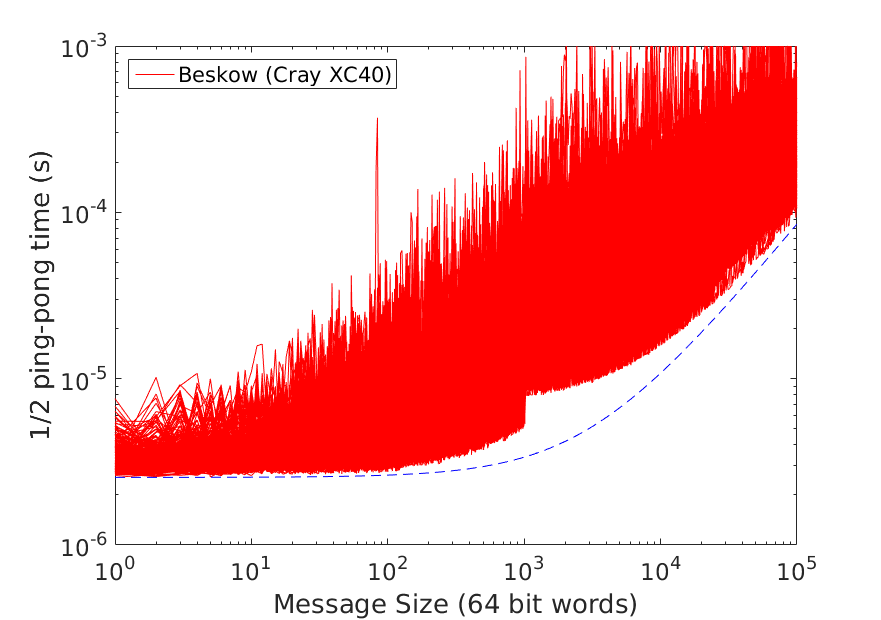
\includegraphics[width=\linewidth]{./figures/pingpong_beskow.png}
  \label{fig:pingpong_beskow}
  }
  \subfigure[Ping-pong on Titan]{
  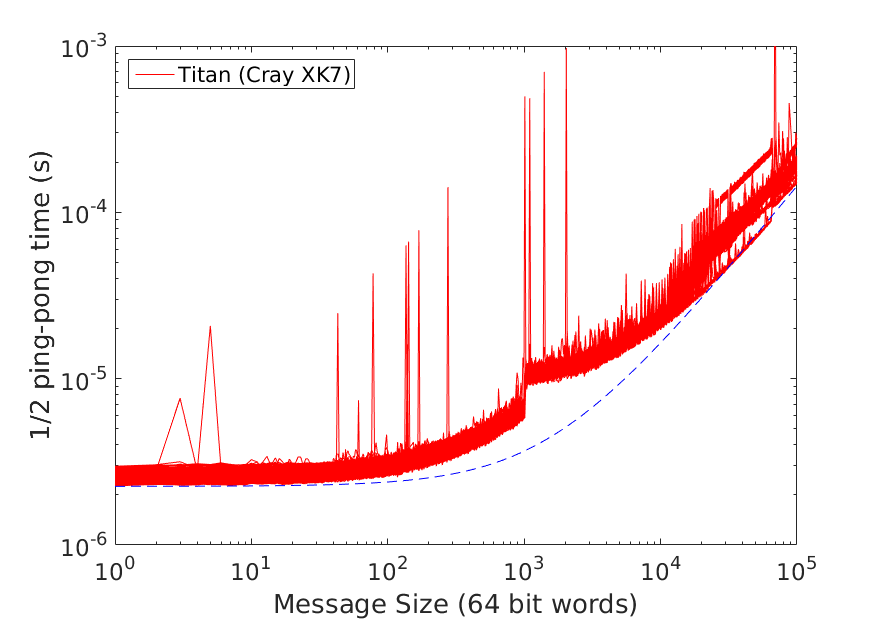
\includegraphics[width=\linewidth]{./figures/pingpong_titan.png}
  \label{fig:pingpong_titan}
  }
  \subfigure[Ping-pong and all-reduce on Mira as illustrated in \cite{fischer:scaling}]{
  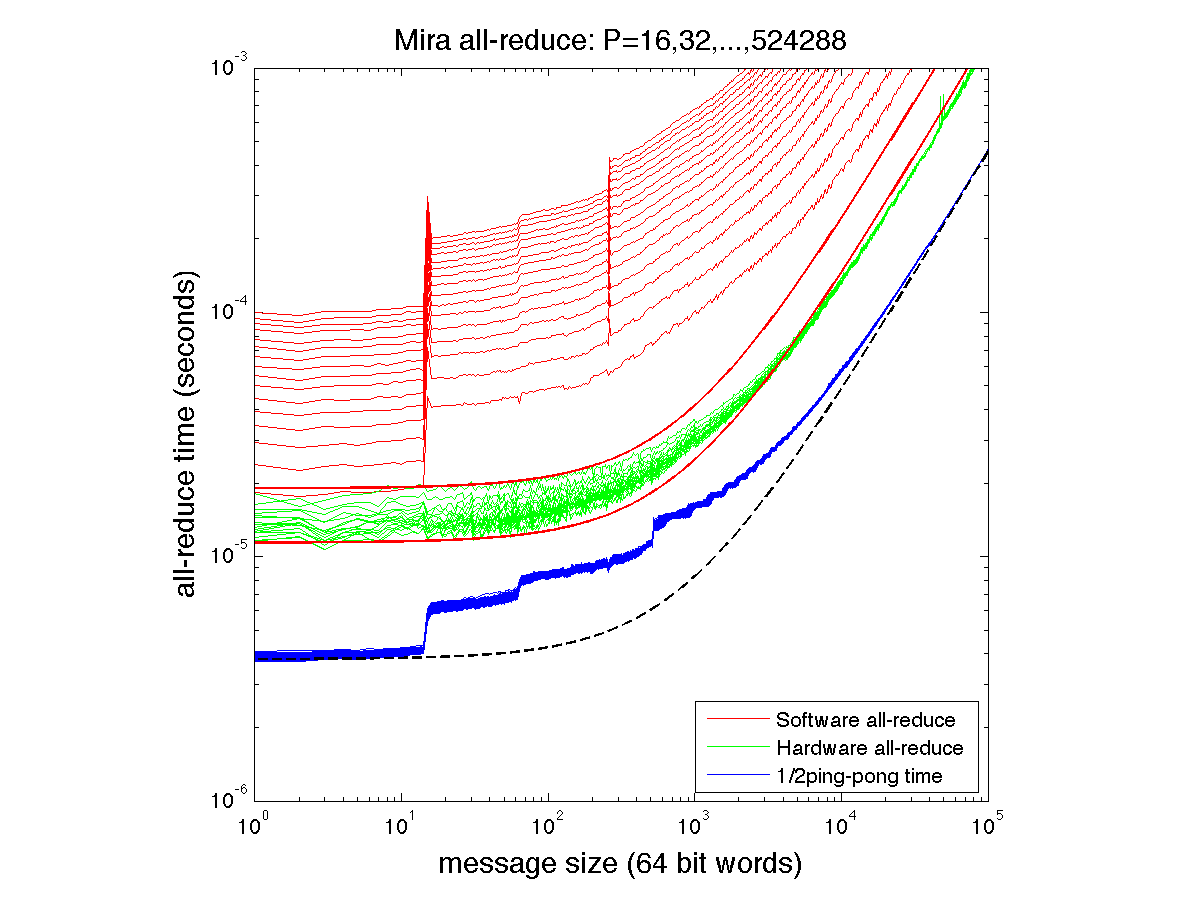
\includegraphics[width=\linewidth]{./figures/pingpong_mira.png}
  \label{fig:pingpong_mira}
  }
  \caption{Latency and Bandwidth Tests on Mira}
  \label{fig:pingpong}
\end{figure}

% Show graph with results of the ping pong test?
% Explain that we took minimum values
% Discuss noise and "randomness" of the results on Cray machines



\section{Nek5000 solver}

\subsection{Method}
projections

\subsubsection{Splitting method}
There are two main solvers available within Nek5000 for computing the solution of incompressible Navier-Stokes, of which one is also ammenable to non-divergence free flows. To preserve generality we picked the latter, based on \cite{Tomboulides1997}, which is in essence a fractional step solver. We solve the following equations
\begin{align}
 \frac{\partial \mathbf{u}}{\partial t} + (\mathbf{u \cdot \nabla}) \mathbf{u} & = - \nabla p + \frac{1}{Re} \nabla^2 \mathbf{u} + \mathbf{f} \label{eqn:NS_momentum},\\
 \nabla \cdot \mathbf{u} & = 0, \label{eqn:NS_continuity}
\end{align}
where $\mathbf{u}$ is the velocity field and $p$ the pressure. The Reynolds number $Re = \frac{U L}{\nu}$ is expressed as a function of a typical velocity scale $U$, length scale $L$ and kinematic viscosity $\nu$. Equations (\ref{eqn:NS_momentum})  and (\ref{eqn:NS_continuity}) are called the continuity and momentum equations respectively. The numerical integration of the momentum equation is done explicitely for the nonlinear convective terms and implicitely for the viscous and pressure term according to \cite{Tomboulides1997}. This method is referred to as $\mathbb{P}_N\mathbb{P}_N$ and leads to the following system of equations for one iteration
\begin {align}
 \mathbf{F} \left( \mathbf{u}^{n} \right) & = \sum_{j=1}^{k} \frac{-b_j}{\Delta t} \mathbf{u}^{n+1-j} + \sum_{j=1}^{k} a_j N \left( \mathbf{u}^{n+1-j} \right) +  \mathbf{f}^{n+1} \label{eqn:rhs1}\\
 \mathbf{\tilde{F}} \left( \mathbf{u}^{n} \right) & = \mathbf{F}\left(\mathbf{u}^{n}\right) + \mu \sum_{j=1}^{k} a_j \left( \nabla \times \left( \nabla \times \mathbf{u}^{n+1-j} \right) \right) \label{eqn:rhs2} \\
 \Delta p^{n+1} & = \nabla \cdot \left( -\frac{b_0}{\Delta t} \mathbf{u}^{n+1} + \mathbf{\tilde{F}} \left( \mathbf{u}^{n} \right) \right) \label{eqn:hmhz_pres}\\
 \Delta \mathbf{u}^{n+1} & = - \frac{b_0}{\Delta t} \mathbf{u}^{n+1} + \nabla p^{n+1} + \mathbf{F} \left( \mathbf{u}^{n} \right). \label{eqn:hmhz_vel}
\end {align}
The nonlinear terms have been gathered in operator $N \left( \mathbf{u}^{k} \right)$. The coefficients $b_k$ and $a_k$ are the coefficients for the explicit discretization of the time derivative and convective terms.

Note to Oana: rewrite in discrete form?? or not
add projections description and reference
explain additive schwarz and link to XXT AMG (ohhh man!!! fun fun fun!)

Equation \ref{eqn:hmhz_pres}, the Poisson equation for the pressure, is the main source of stiffness and its efficient resolution by iterative solver is preceded by two steps. First of all, the pressure at each time iteration is projected onto a subspace of previous solutions and serves as first guess for the iterative solver. We used a subspace of length $20$ in the present case. This method, described in \ref{tufo:terascale} (right paper?), has been shown to reduce the iteration count by a factor $2.5-5$. Then, A pressure preconditioner is built based on the additive overlapping Schwarz method and a coarse grid solve. Is is given by 
\begin{equation}
 M_0^{-1} := R_0^T A_{0}^{-1} R_0 + \sum_{k=1}^{K} R_k^T \tilde{A}_k^{-1} R_k.
\end{equation}
The overlapping part require local solves on each subdomain and is easily parallelized \cite{Fischer199784,Fischer2005}. The coarse grid solve is more difficult to parallelize and can be performed in two different ways. The first method is XXT \cite{Tufo2001151}, where the solution on the coarse grid is projected on a basis that constitutes a quasi-sparse factorization of $A_0^{-1}$. The second method is an algebraic multigrid solver (AMG) that operates a smoothing, a coarsening and a interpolation operation on a predefined number of coarse grid levels. Finally, the pressure equatin is solved with the generalized minimal residual method (GMRES).

In a similar way, Equation \ref{hmhz_vel}, the Poisson equation for the velocity, is solved using the conjugate gradient (CG) iterative solver but without the need for a Schwarz method or a coarse grid solve.
% \begin{align}
%  \mathbf{u}_i^* & = \beta_0 \mathbf{u}_i^n + \beta_1 \mathbf{u}_i^{n-1} + \beta_2 \mathbf{u}_i^{n-2}, \label{eqn:extrap_vel}\\
%  \mathbf{h}_i^n & = N(\mathbf{u}_i^n) + B \mathbf{f}_i + ???, \label{eqn:rhs}\\
%  A \delta \mathbf{p}^n & = \nabla \cdot \left[ \left( \sum_{i=1}^3 \frac{-1}{Re} (\nabla \times (\nabla \times \mathbf{u}_i^*)) + B^{-1} \mathbf{h}_i^n \right) \right]\nonumber\\
%  & \quad - A \mathbf{p}^n , \label{eqn:hmhz_pres} \\
%  A \delta \mathbf{u}^{n} & = -A \mathbf{u}^{n} + \mathbf{h}_i^n \label{eqn:hmhz_vel},\\
%  \mathbf{p}^{n+1} &= \mathbf{p}^{n} + \mathbf{\delta p}^{n}, \label{eqn:update_p} \\
%  \mathbf{u}_i^{n+1}& = \mathbf{u}_i^{n} + \mathbf{\delta u}_i^{n}.  \label{eqn:update_u} 
% \end{align}
% The operators $A$ and $B$ represent the discrete Laplacian operator and the mass matrix respectively. The index $i=1,2,3$ represents the 3 spatial directions $x$, $y$ and $z$. The intermediate velocity $\mathbf{u}_i^*$ is extrapolated using a third order Adams-Bashforth scheme in Equation (\ref{eqn:extrap_vel}). The corresponding coefficients $\beta_k$ are given by $\beta_0 = \frac{23}{12}$, $\beta_1 = \frac{-4}{3}$ and $\beta_2 = \frac{5}{12}$ (??). The term $\mathbf{h}_i^n$ from equation (\ref{eqn:rhs}) contains the nonlinear convective term $N(\mathbf{u}_i^n)$ evaluated explicitely, the external forcing $\mathbf{f}_i$ and ???. Equation (\ref{eqn:hmhz_pres}) is solved using a Generalized minimal residual method (GMRES), while equation (\ref{eqn:hmhz_vel}) is solved using the conjugate gradient (CG) mehtod. Furthermore, both the pressure and velocity vectors are projected onto a space of previous solutions in order to speed up the convergence of the iterative solvers. Projections occur before and after the 
% iterative solver. %When solving equations (\ref{eqn:hmhz_pres}) and (\ref{eqn:hmhz_vel}), we obtain the corrections for the pressure and the velocity that we can use to update those variables in Equations \ref{eqn:update_p} and \ref{eqn:update_u}.

%\subsubsection{Coarse grid solver}

% introduce coarse grid solver for the pressure
\section{Prior Work}
Link to the complexities in the Fischer paper -> multiplicities
Explain finite difference link

\subsection{Implementation}
\label{sec:implementation}
The geometry is meshed using hexahedral elements, partioned for parallel computation using a spectral bisection algorithm as implemented in "genmap" which accompanies the code Nek5000 (insert ref documentation and check if the genmap description is still in.. and give it to gail for once!!!!)
\begin{figure}
  \centering
  \subfigure[Partition]{
  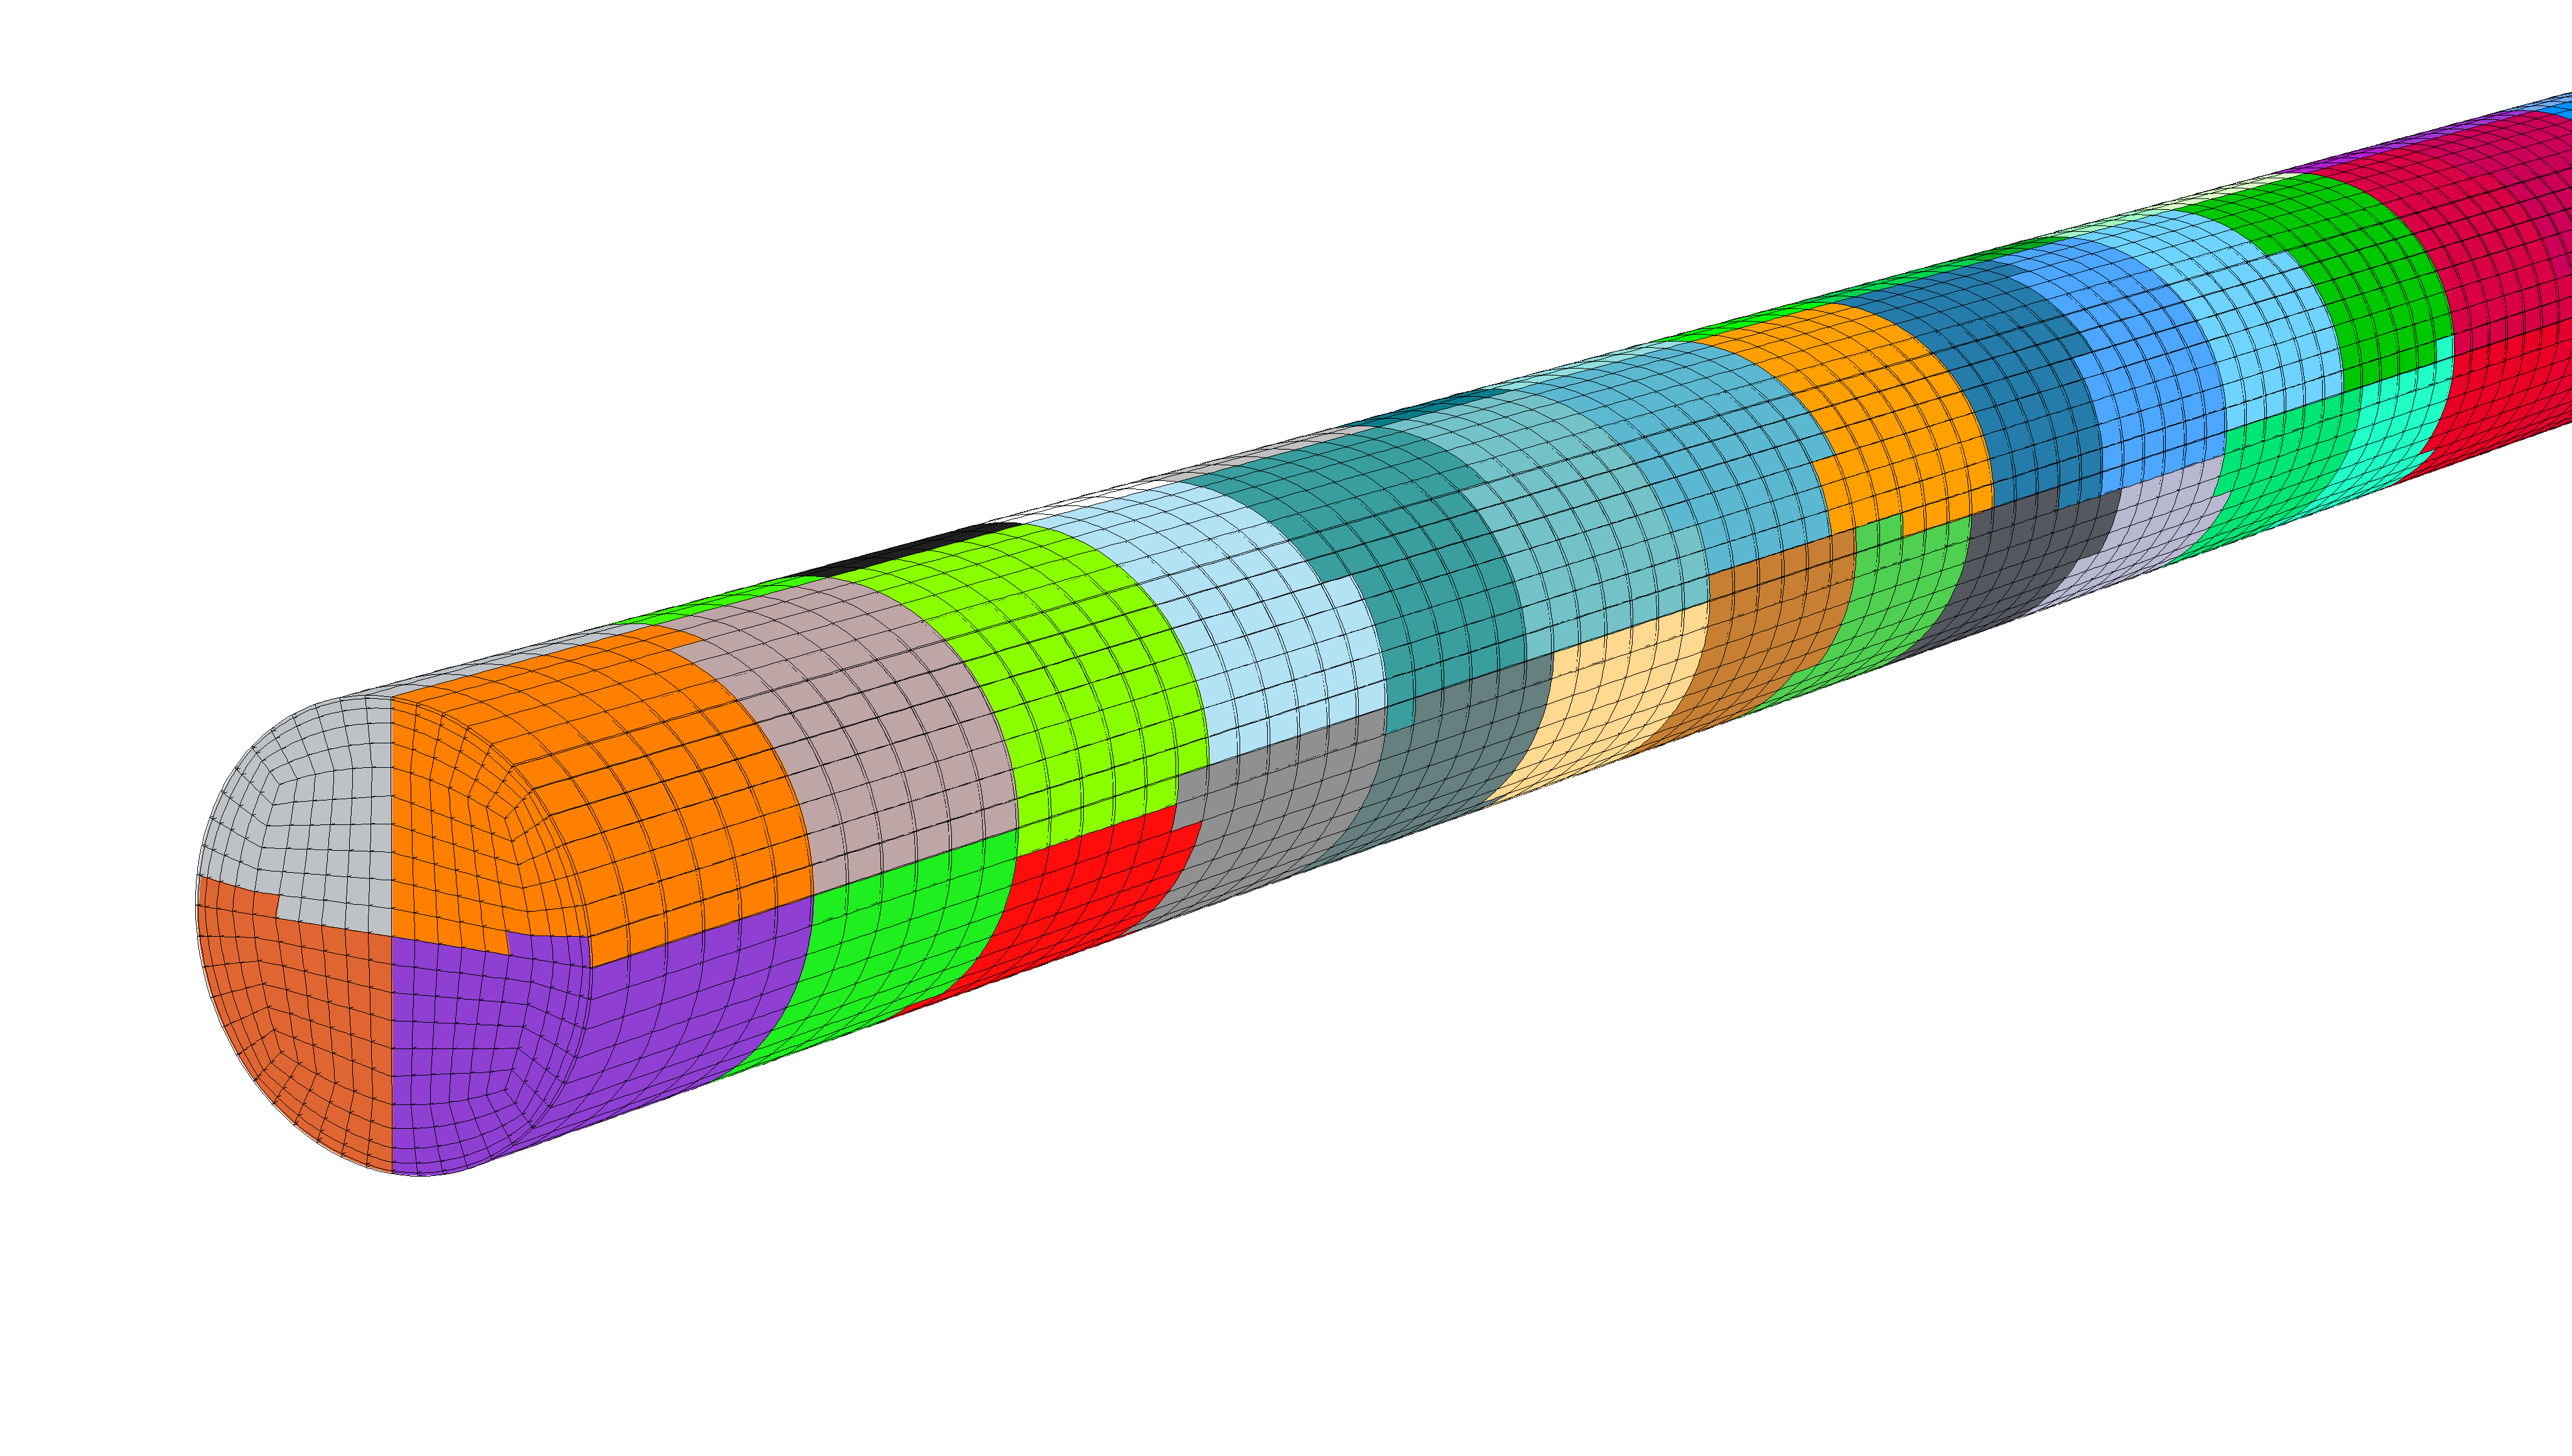
\includegraphics[trim=300 400 800 350,clip,width=\linewidth]{./figures/partition2.png}
  }
  \subfigure[Velocity magnitude]{
  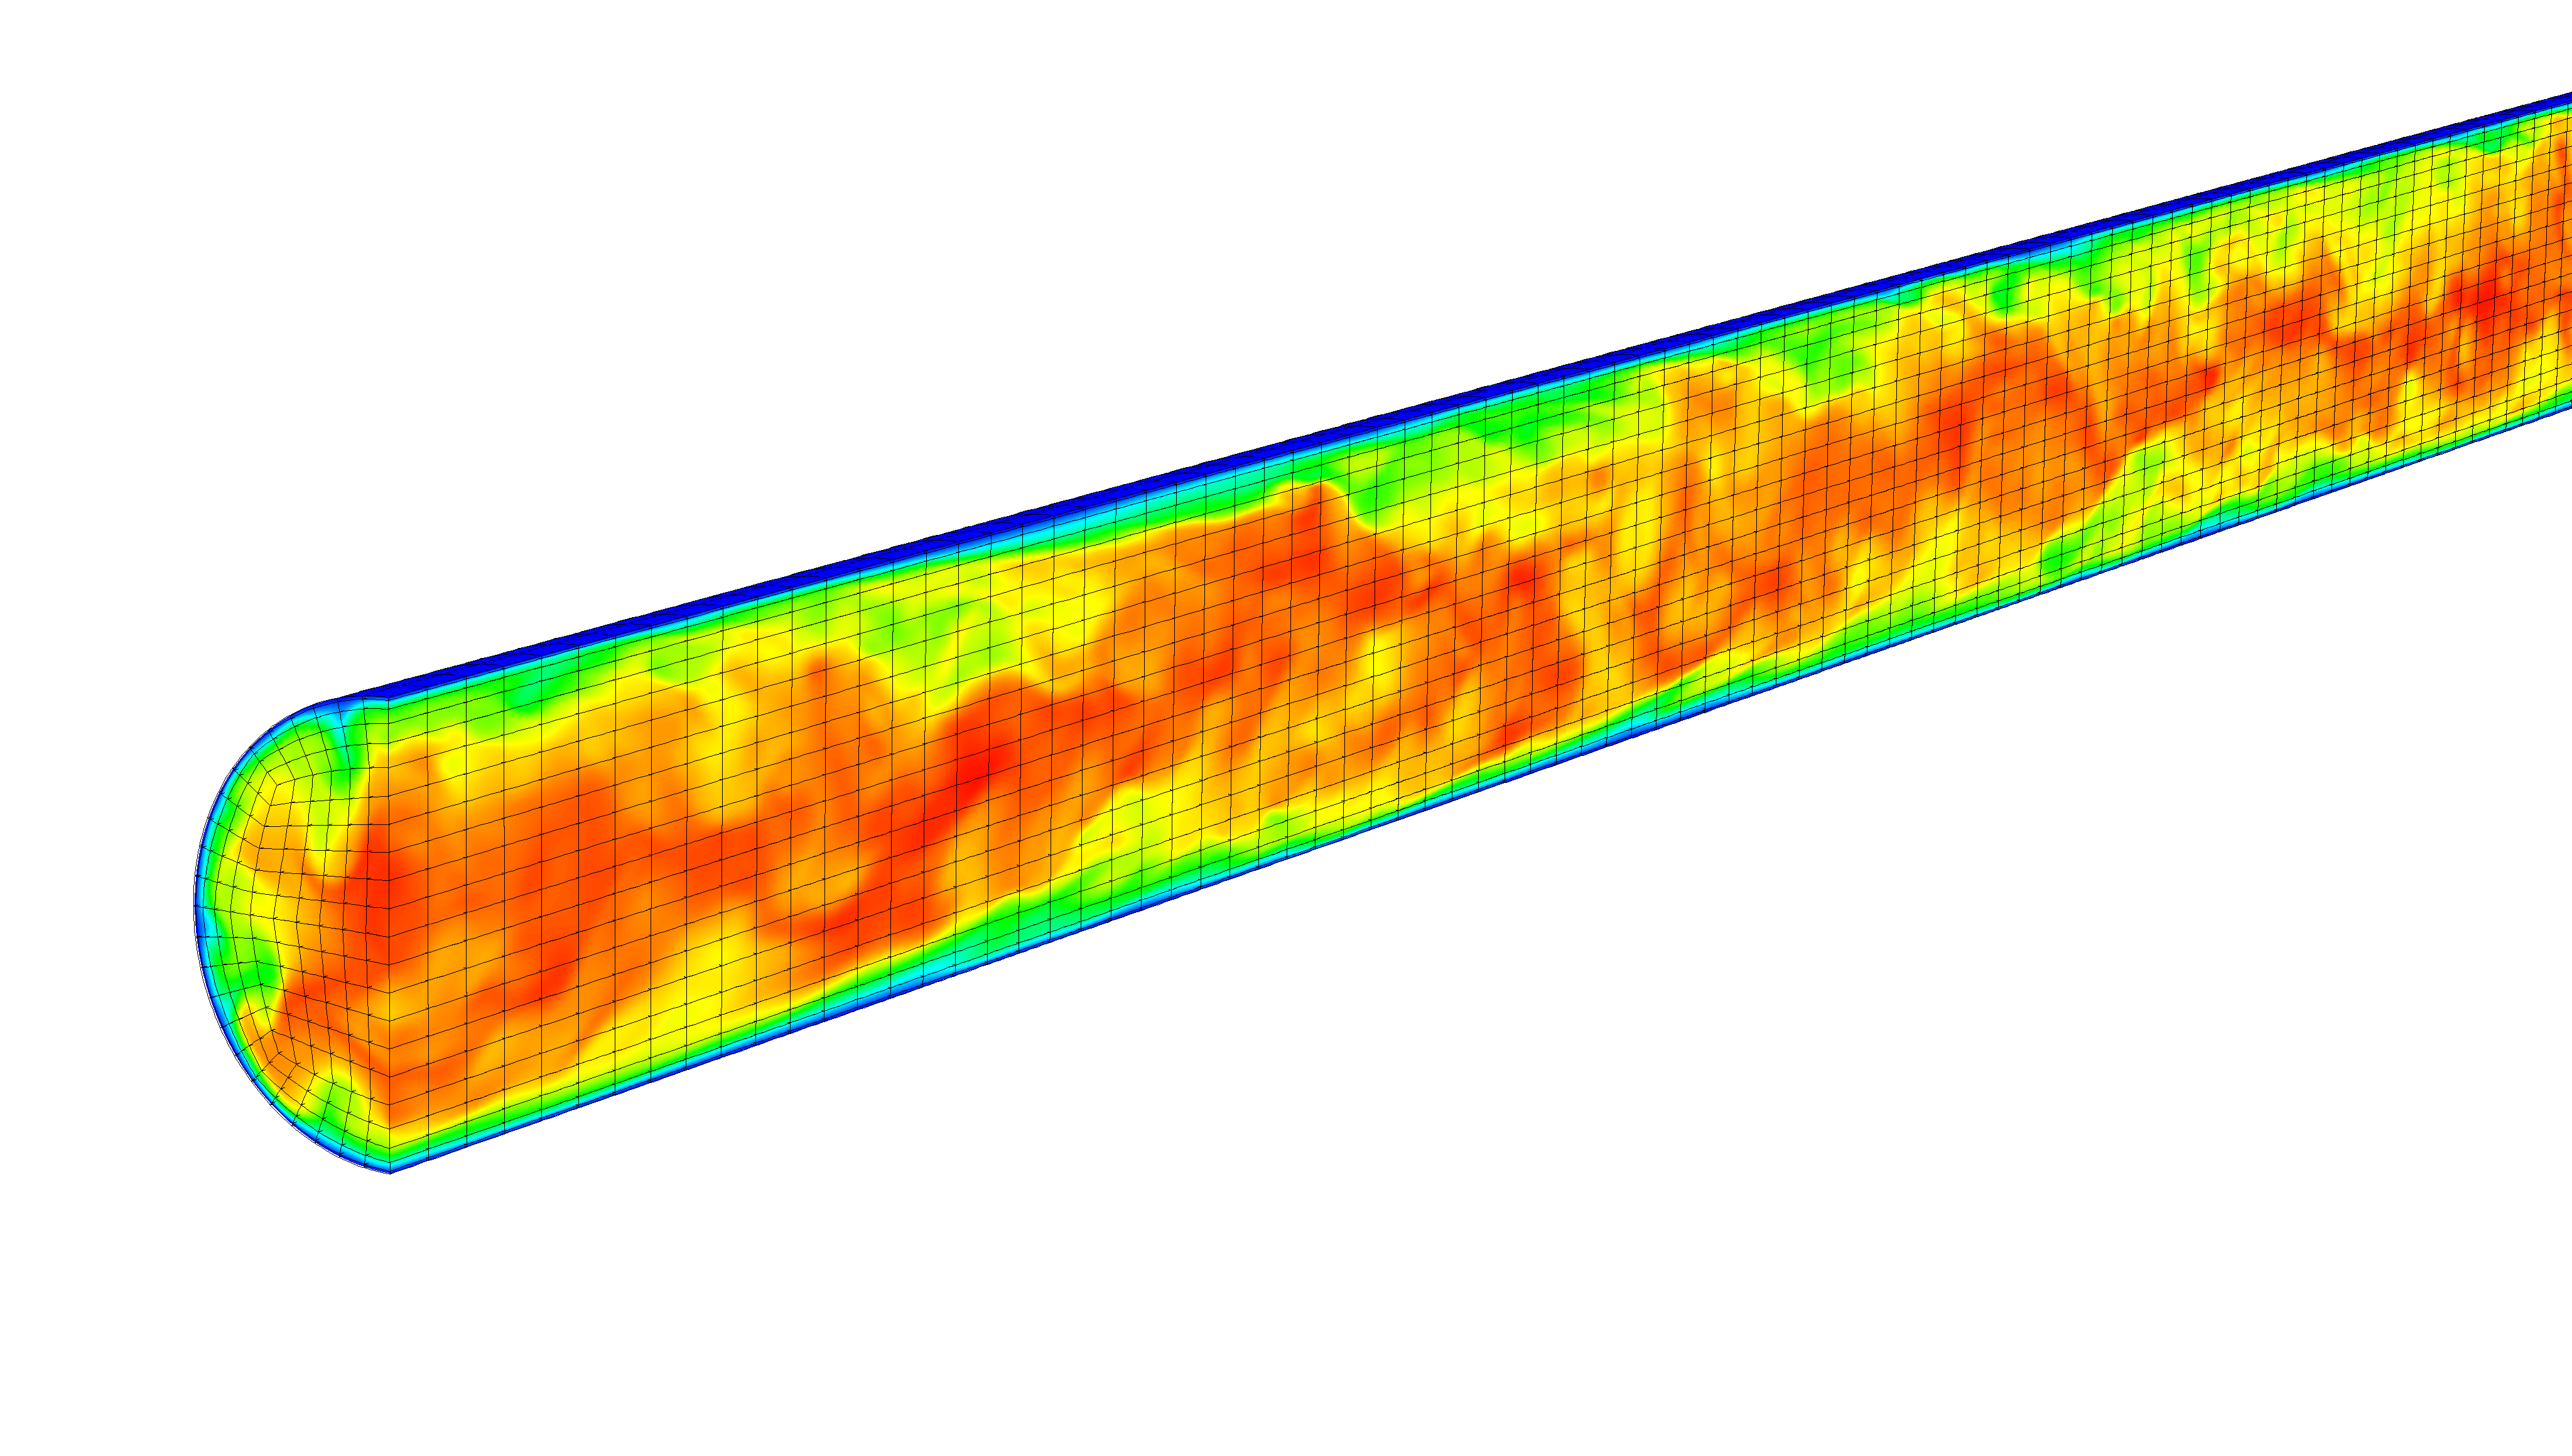
\includegraphics[trim=300 400 800 350,clip,width=\linewidth]{./figures/vel_magn.png}
  }
  \caption{Partition of the elements and velocity magnitude in the pipe ($Re_{\tau}=180$).}
  \label{fig:partition}
\end{figure}
 
I should have next to the partition figure the flow at same angle and size, possible Nicolas? 
\subsubsection{Code structure}
\label{sec:code}

The main loop iterates over the time steps. At each time step, the pressure is solved first and then the velocity components. Furthermore, each of those fields is projected before and after being solved. The pressure is solved with the GMRES method while conjugate gradient is used for the velocity. The pressure solve also includes the computation of the preconditioner based on the Schwarz overlapping method and coarse grid solve, which is not the case for the velocity and constitutes an important part of the work and communication.

\subsubsection{Instrumentation for the Timers}
\label{sec:timers}
Our strategy for timing the code execution is twofold. For one, we use MPI
timers for the wall clock time and profiling libraries that were deemed suitable
for our use case. We are running the code on our test case (see
\refsec{sec:pipe}) after a full restart for 50 time steps. We save 5 past
projections and are measuring the time from the 30th to the 50th time step; in
total 20 time steps. 
\paragraph{MPI Timers}
Based on the structure presented in \refsec{sec:code} we placed 9 timers in the code that are
only switched on during the last 20 time steps. Each timer measures the wall
clock time using the MPI timer ({\tt MPI\_Wtime}) followed by a barrier
({\tt MPI\_Barrier}) guaranteeing coherent and synchronized measurements. We
have run the code without synchronization and timers to evaluate the created
overhead due to our measurements. In all instances this overhead has been far
below 5\%. The main timer computes the total time spent in the outer timestepping loop for the last 20 timesteps. Then, we have timers for the compute time of $\mathbf{F} \left( \mathbf{u}^{n} \right)$, i.e.\ the right hand side of equation (\ref{eqn:rhs1}) and the right hand side of equation (\ref{eqn:hmhz_pres}). We also time all the different projections separately, using 4 timers (one timer before solving and one after for both pressure and velocity). The time spend in the Helmholtz solves is measured as well for pressure and velocity. Within the pressure solver, we put a timer around the coarse grid solve. Finally, we gather in an additional timer most of the remaining computations such that our timers account for more that 95\% of the total time. We learn from these timers that the projections are in most cases the most time consuming functions, followed by the Helmholtz solves. However, these timers do not provide information about the repartition between the time spent in computation and communication, which is the core element when assessing scalability and efficiency of a parallel code. Therefore, we do not present the results obtained with those timers and instead investigate in more details the timings produced by more adapted sampling and profiling tools.
\paragraph{Craypat and Hardware Performance Monitor}
In order to measure the time spent in communication we relied on Craypat for
Beskow and Titan and on Hardware Performance Monitor (HPM) for Mira. Both tools
allow us to measure the total time spent in communication during the targeted 20 time
steps. In addition HPM gives additional information on the cache misses and the load
imbalance. The CrayPat performance analysis framework is used to sample the code during execution at a default frequency of $\unit[100]{Hz}$ and reports in which function each sample was taken. Then, we assume that the proportion of the total time spent in a given function is equal to the proportion of samples within this function. The sampling procedure ensures a very low overhead. We also tested the profiling procedure, where all function calls are tracked, available with Craypat but overhead in time was about $50\%$ and the method was abandoned.

%\subsection{Models for parallel performance}

%\subsubsection{Computational complexity}

%\subsubsection{Communication model}

% In practice, each simulation is restarted from a previously computed turbulent solution and is run during $50$ time steps. The projections for velocity and pressure are turned on after $5$ time steps, the number of the previous pressure solutions saved is $20$ and the timers are turned on during the last $20$ time steps. Therefore, heavy input/output is not included and projections are working fully during the measurement period.

% Present system of equations
% Describe briefly the algorithm behind nek
% Mention and discuss PN-PN
% Discuss the two coarse grid solver XXT and AMG

\section{Performance and Scaling Analysis}
\label{sec:analysis}
Notes: c32
Large scale runtime performance is influenced by 
\begin{enumerate}
  \item Network topology
  \item Time $T_a$ and $T_c$ spent in computation and communication,
    %respectively
  \item ratio of runtime and communication times: $r \leq \dfrac{T_a}{T_c}$,
  \item degrees of freedom $N$ per process $P$: $\dfrac{N}{P}$,
  \item partitioning imbalance.
\end{enumerate}

We will measure the load imbalance, cache misses, multiplicities of grid points
across as well as weak and strong scaling.
While relying on the results of \cite{tufo:terascale}, we want in particular to verify
experimentally the strong scaling limit which is defined as the ratio of $\dfrac{N}{P}$ where
$\dfrac{T_a}{T_c}\leq 1$ inequality is equal to $1$ with increasing $P$. The
abstraction of communication and computation time does not take into account
factors as load imbalance, cache misses or accelerated collective communications.

The communication is subdivided into nearest neighbour (NN) and so called
allreductions. As the NN hints, the communication takes place between a spatial
partition and all of its neighbours. In a 3D cubic with cubic partitioning this
would be 8 for the vertices, 4 for the edges and 2 for the faces. We assume that
all NN on mesh are also nearest neighbours on the partitioning mapped to the
physical topology of the hardware. We will prove in \refsec{sec:abstractions}
that our use case presented in the next section is equivalent to a cubic
partitioning and rely on the complexities of \cite{fischer:scaling} for $T_c$ and
$T_a$. The performance of allreduce is a core indicator of a system's
performance and is dependent on its network hardware. The most prevalent
complexities for allreductions are given by $\bigo{\dfrac{n}{P}\cdot \log(P)}$. All
systems used in this paper rely on accelerated allreduce MPI communication that have
a complexity of $\bigo{n}$, independently of $P$. Beskow uses the dragonfly
topology where accelerated collectives are being presented in
\cite{jain2012collectives}. Titan and Mira use a 3D and 5D torus, getting the
reduction cost down to $\alpha \cdot c \cdot n$ where $c$ is a low constant
value. In the end, the collective communication is the dominant and
differentiating factor in the scaling behavior of Nek on those three systems.

A generic case, widely known across the CFD community, is used to explore the
scaling behavior of Nek. This should allow potential users to estimate and
compare the scaling of Nek to other CFD software.
\subsection{Test Case: Pipe}
\label{sec:pipe}

The test case considered is the turbulent flow in a straight pipe. A thorough description of the flow configuration as well as a detailed analysis of the physical results can be found in \cite{Khoury2013}. The flow was run at four different friction Reynolds numbers $Re_{\tau} = 180$, $360$, $550$ and $1000$. A summary of the different simulations and associated number of elements and number of grid points is presented in Table \ref{tab:pipe_conf}. The friction Reynolds number is defined as $Re_{\tau} = u_{\tau} R / \nu$, where $u_{\tau}$ is the friction velocity $R$ is the radius of the pipe and  $\nu$ is the kinematic viscosity. The bulk Reynolds number is defined as $Re_{b} = 2 U_b R / \nu$, where $U_b$ is the mean bulk velocity. 

\begin{table}
\centering
\caption{Summary of the different pipe flows configurations.}
\begin{tabular}{llrr} 
\hline
$Re_{\tau}$&$Re_{b}$&\# of elements & \# of grid points\\ 
\hline
$180$ & $5300$ & $36,480$ & $18.67 \times 10^6$\\
$360$ & $11,700$ & $237,120$ & $121.4 \times 10^6$\\ 
$550$ & $19,000$ & $823,632$ & $437.0 \times 10^6$\\ 
$1000$ & $37,700$ & $1,264,032$ & $2.184 \times 10^9$\\
\hline
\end{tabular}
\label{tab:pipe_conf}
\end{table}
%\subsection{Abstractions and Assumptions}
%\label{sec:abstractions}
%\subsubsection{$\alpha$, $\beta$}
%\subsubsection{Imbalance}
%\subsubsection{Weak/Strong Scaling, Efficiency}
%\subsubsection{Cache Misses and Scaling}
%\subsubsection{Partitioning and Imbalance}


\section{Results}

Our four test cases were run with various processor counts on three systems. The
lower bound for the processor count is given by the amount of RAM to fit a given
problem into memory. Nek5000 has roughly a memory requirement of 500 fields
times the number of degrees of freedoms. The upper bound was either due to the
administrative limit of getting access to the maximum number of processors
(Beskow and Titan) or by the limit of having 1 or 2 elements per process. As has
been pointed out in \refsec{sec:code}, the parallelization of Nek5000 is at the
element level so that one element may not be partitioned further. 
As anticipated in \refsec{sec:timers}, we measure the communication time and
computation time of the chosen 20 timesteps. 

In \cite{fischer:scaling} the strong scaling limit where $r=\dfrac{T_a}{T_c}=1$ was estimated
to be at about $\frac{n}{P}=2000$ for the conjugent gradient (CG) and $20000$ or
$7000$ (BG/Q) for the algebraic multigrid (AMG). As described in \refsec{sec:code}, the
Nek5000 solvers XXT and PNPN consist of several CG and AMG solves. Furthermore,
there is an overhead for the setup, the projections, the coarse solve and other
none runtime relevant components. Moreoever, the convergence of the underlying
algorithms is also very case dependent, thus influencing the overall runtime
behavior. Our runtimes give an overall impression of the Nek5000 behaviour on
various systems based on a generic well known case in CFD (see
\refsec{sec:pipe}). 

The scaling plots for all three
systems in \reffig{fig:mira} and \reffig{fig:beskow} are the fundamental
measurements for our further analysis of the weak/strong scaling, computation
versus communication time and load imbalance.
\begin{figure}
  \centering
  \subfigure[$Re_{\tau} = 180$]{
  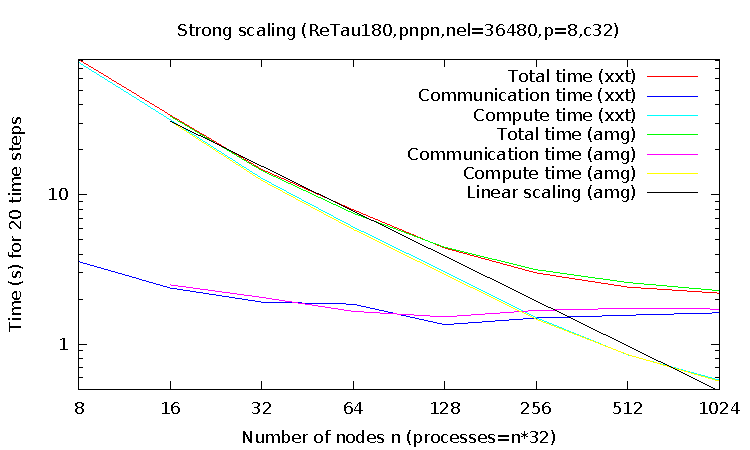
\includegraphics[width=\linewidth]{./figures/mira/scaling_ReTau180.pdf}
  }
  \subfigure[$Re_{\tau} = 360$]{
  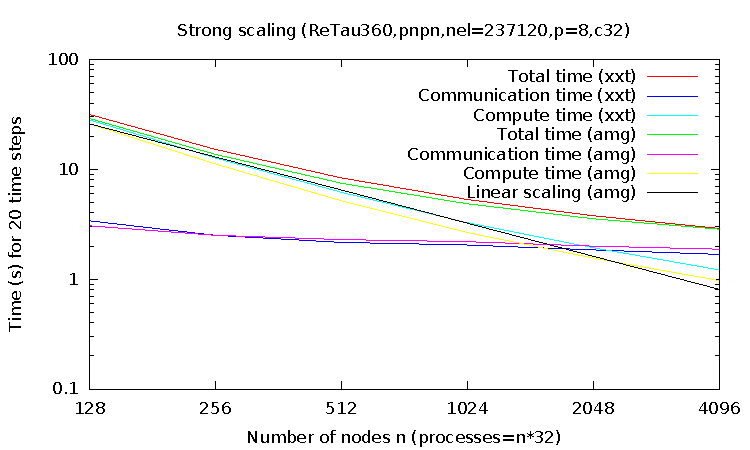
\includegraphics[width=\linewidth]{./figures/mira/scaling_ReTau360.pdf}
  }
  \subfigure[$Re_{\tau} = 550$]{
  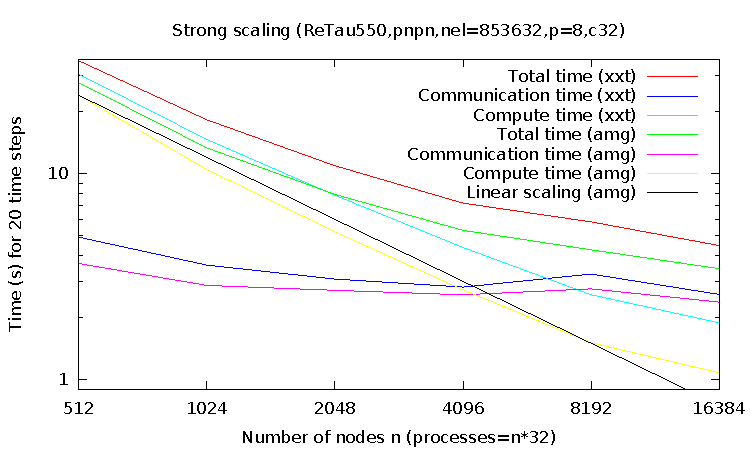
\includegraphics[width=\linewidth]{./figures/mira/scaling_ReTau550.pdf}
  }
  \subfigure[$Re_{\tau} = 1000$]{
  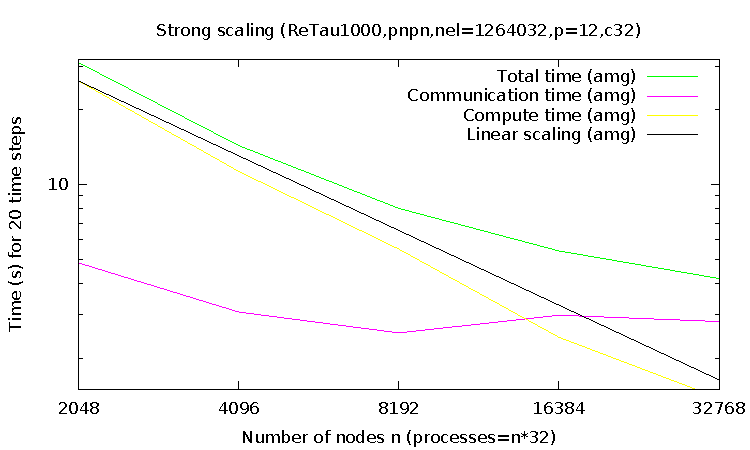
\includegraphics[width=\linewidth]{./figures/mira/scaling_ReTau1000.pdf}
  }
  \caption{BG/Q Mira}
  \label{fig:scaling_mira}
\end{figure}

\begin{figure}
  \centering
  \subfigure[$Re_{\tau} = 180$]{
  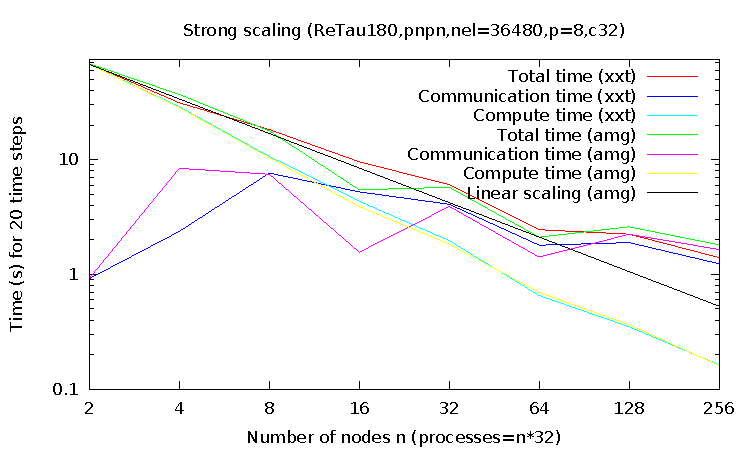
\includegraphics[width=\linewidth]{./figures/beskow/scaling_ReTau180.pdf}
  }
  \subfigure[$Re_{\tau} = 360$]{
  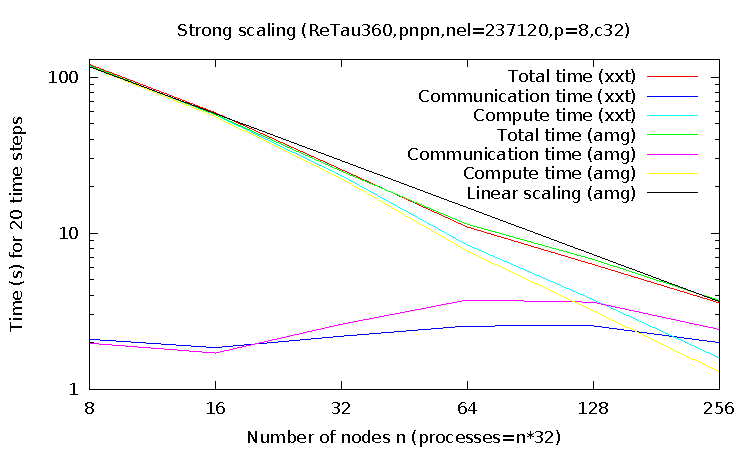
\includegraphics[width=\linewidth]{./figures/beskow/scaling_ReTau360.pdf}
  }
  \subfigure[$Re_{\tau} = 550$]{
  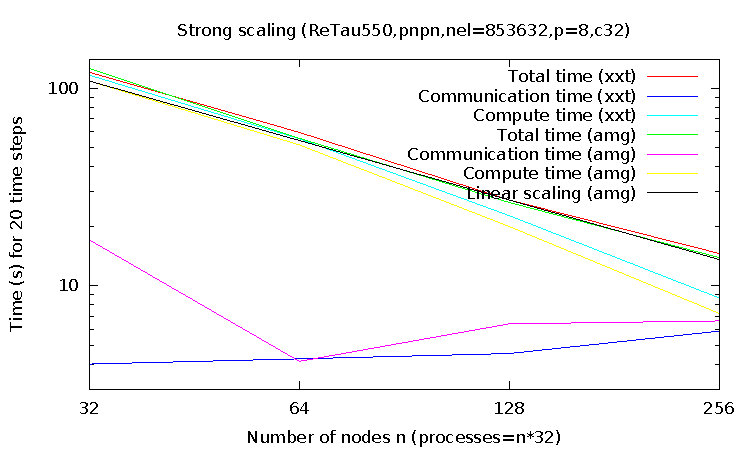
\includegraphics[width=\linewidth]{./figures/beskow/scaling_ReTau550.pdf}
  }
  \subfigure[$Re_{\tau} = 1000$]{
  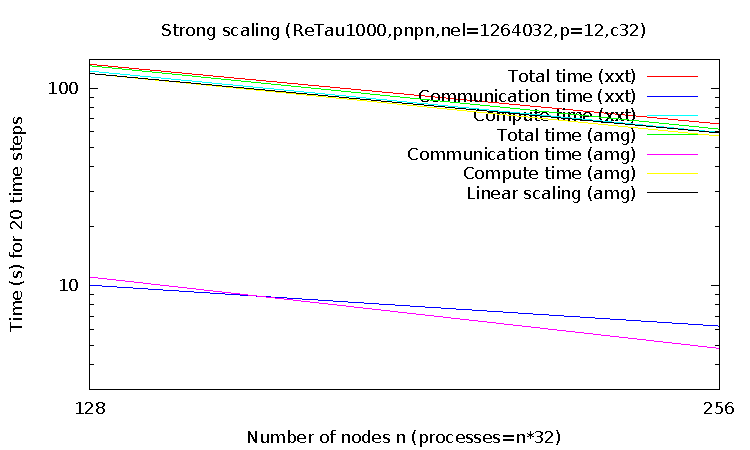
\includegraphics[width=\linewidth]{./figures/beskow/scaling_ReTau1000.pdf}
  }
\caption{Beskow}
\label{fig:scaling_beskow}
\end{figure}

\begin{figure}
  \centering
  \subfigure[$Re_{\tau} = 180$]{
  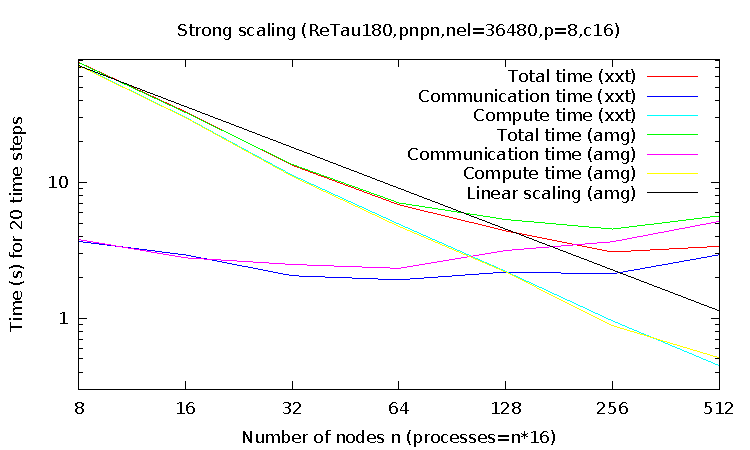
\includegraphics[width=\linewidth]{./figures/titan/scaling_ReTau180_titan.pdf}
  }
  \subfigure[$Re_{\tau} = 360$]{
  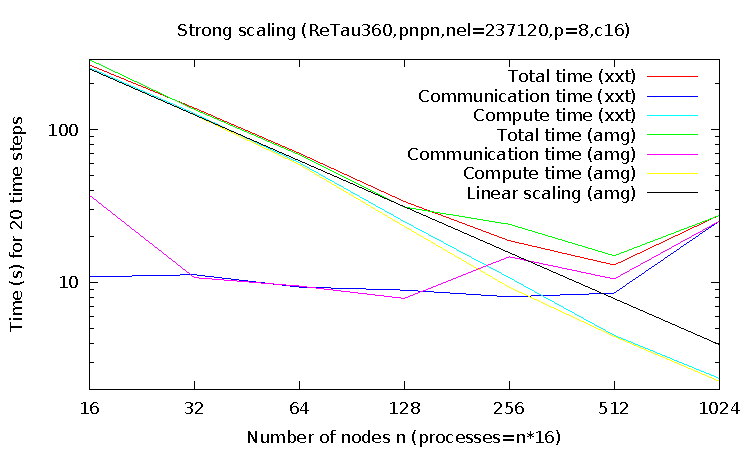
\includegraphics[width=\linewidth]{./figures/titan/scaling_ReTau360_titan.pdf}
  }
  \subfigure[$Re_{\tau} = 550$]{
  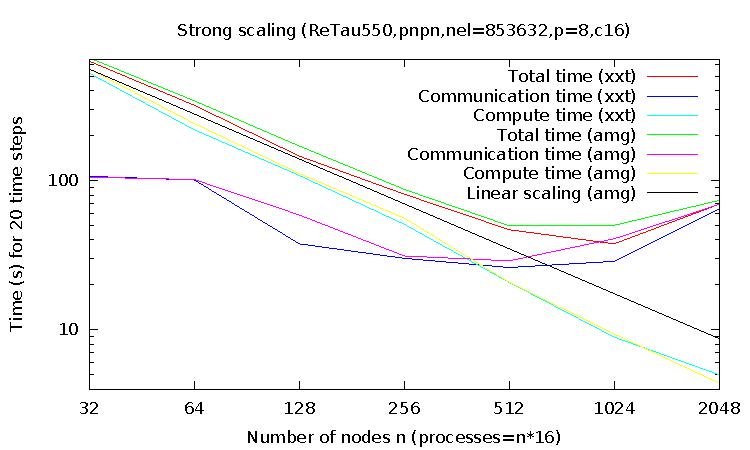
\includegraphics[width=\linewidth]{./figures/titan/scaling_ReTau550_titan.pdf}
  }
  \subfigure[$Re_{\tau} = 1000$]{
  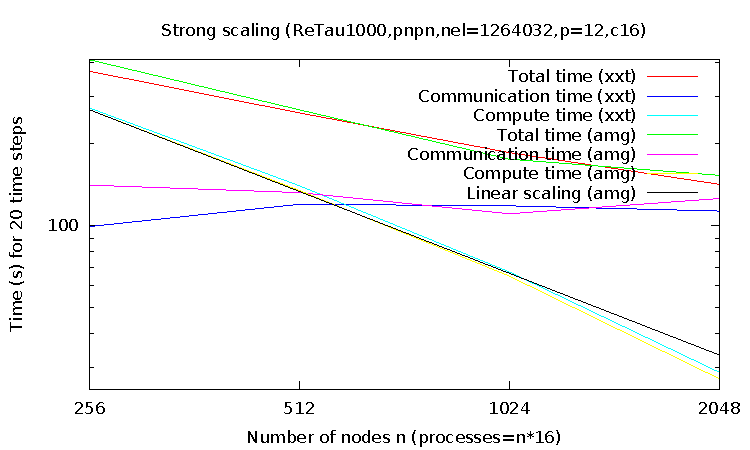
\includegraphics[width=\linewidth]{./figures/titan/scaling_ReTau1000_titan.pdf}
  }
\caption{Titan}
\label{fig:scaling_titan}
\end{figure}

\begin{figure}
  \centering
  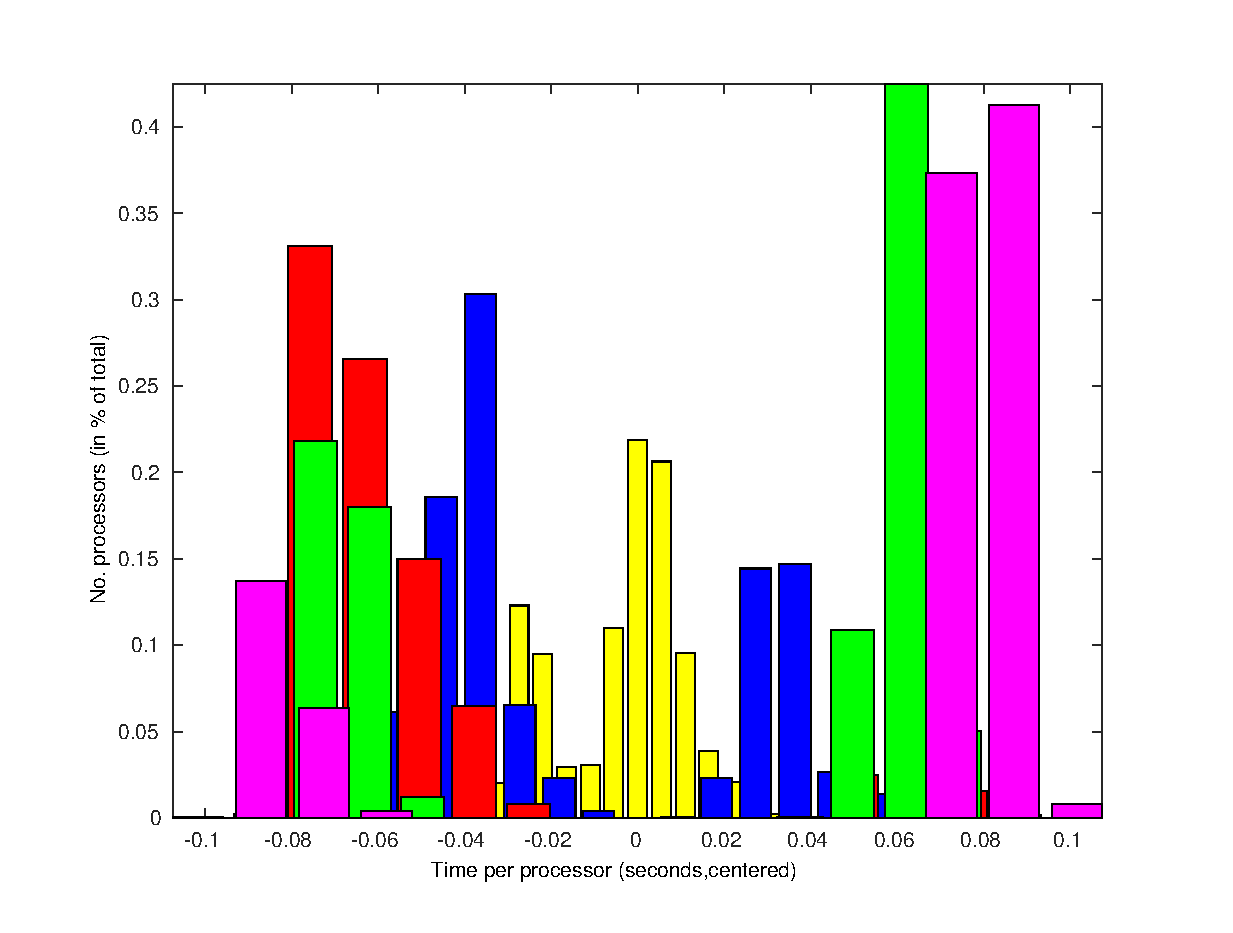
\includegraphics[width=\linewidth]{./figures/imbalancehist.eps}
  \caption{Histogram of the load imbalance}
  \label{fig:imbalancehist}
\end{figure}


\subsection{Weak and Strong Scaling}

The ratio of computation and communication time $r=\frac{T_a}{T_c}$ is a key
indicator for the strong scaling limit. If communication takes longer than
computation, the code is deemed to be at the strong scaling limit where the
scaling diverges significantly from the perfect linear scaling. For both XXT and
AMG this point is clearly determined in the plots where the computation time
crosses the communication time. 

On Mira this limit has consistently in all 4 cases (see
\reffig{fig:scaling_mira}). The approximations of values for $\frac{n}{P}$ where
$r=1$ are listed below:
  
\begin{tabular}{ccccc}
  &ReTau180&ReTau360&ReTau550&ReTau1000\\
  XXT&2300&1900&2000&\\
  AMG&2300&2400&3300&4000\\
\end{tabular}

In practice we observed a strong scaling limit $r=1$ for XXT at roughly $1900<
\frac{n}{P} < 2300$ and for AMG at $2300<\frac{n}{P}<4000$, below the $7000$
anticipated in \cite{fischer:scaling}. 

In theory the compute time scaling should exactly match linear scaling
as computational work is distributed according to the ratio $\frac{n}{P}$. All
algorithms in Nek5000 should yield little overhead due to the halo update. 

\begin{figure}
  \centering
  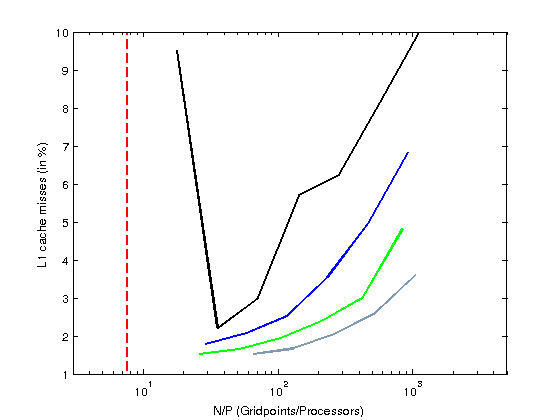
\includegraphics[width=\linewidth]{./figures/cachelines.png}
  \caption{Cache Misses}
  \label{fig:cachemisses}
  \caption{Cache misses on Mira for all 4 test cases are decreasing with
  decreasing degrees of freedom per process. For $Re_{\tau}=180$, we observe a
  sudden spike at the run with 1 element per process. The dashed red line is the
  cache size after which all gridpoints would theoratically fit into cache.}
\end{figure}

All test cases on all the systems show a super linear scaling. This
observation holds true with all timers and profilers switched off.
Numerically there is no explanation for this behavior. 

The usual explanation for super linear scaling are a sudden decrease of the cache
misses for decreasing $\frac{n}{P}$, as parts of the solver can entirely work on
data that lies in the cache. 
To investigate this, we extracted the cache misses on Mira provided by HPM (see
\reffig{fig:cachemisses}). Mira is equipped with L1 cache of 16kb. The L2 cache
of 32mb, that is located at the node level, is irrelevant as we had consistently
over 97\% cache misses. The L1 cache can be filled with $2048$ double precision
numbers. As we run with 2 processes per core, this would be at roughly 1000
degrees of freedom per process. Although the data fields achieve those sizes only at the strong scaling
limit we do observe a general decrease in cache misses with decreasing
$\frac{n}{P}$. The only exception is the test case for $Re_{\tau}=180$ where we
have a sudden spike in cache misses where we run at one element per core. This
is the only run that was performed at a process count that is not to the power
of two.
In summary, we attribute the super linear scaling to cache
management and pipelining on the CPU of Mira. 

Beyond the strong scaling limit, the computation time increases again and
approaches the linear scaling line again. This is attributed to the load
imbalance as in the extreme case some processes have to work on one element and
some processes on two elements. This can be observed in \reffig{sec:imbalance}
where the imbalance for $Re_{\tau}=1000$ on 32768 nodes creates two spikes in the
distribution of the execution time. The histogram includes the imbalance of
workload as well as the resulting imbalance in the communication.

On Mira the communication is mostly latency bound with a small influence of the
bandwidth. This holds true for peer to peer communication as well as for the
all-reduce (see \reffig{fig:pingpong}).

Across the four test cases we can observe a weak scaling in
\reffig{fig:weakscaling}. It proves that the scaling on Mira is only dependent
on the ratio $\frac{n}{P}$. 
\begin{figure}
  \centering
  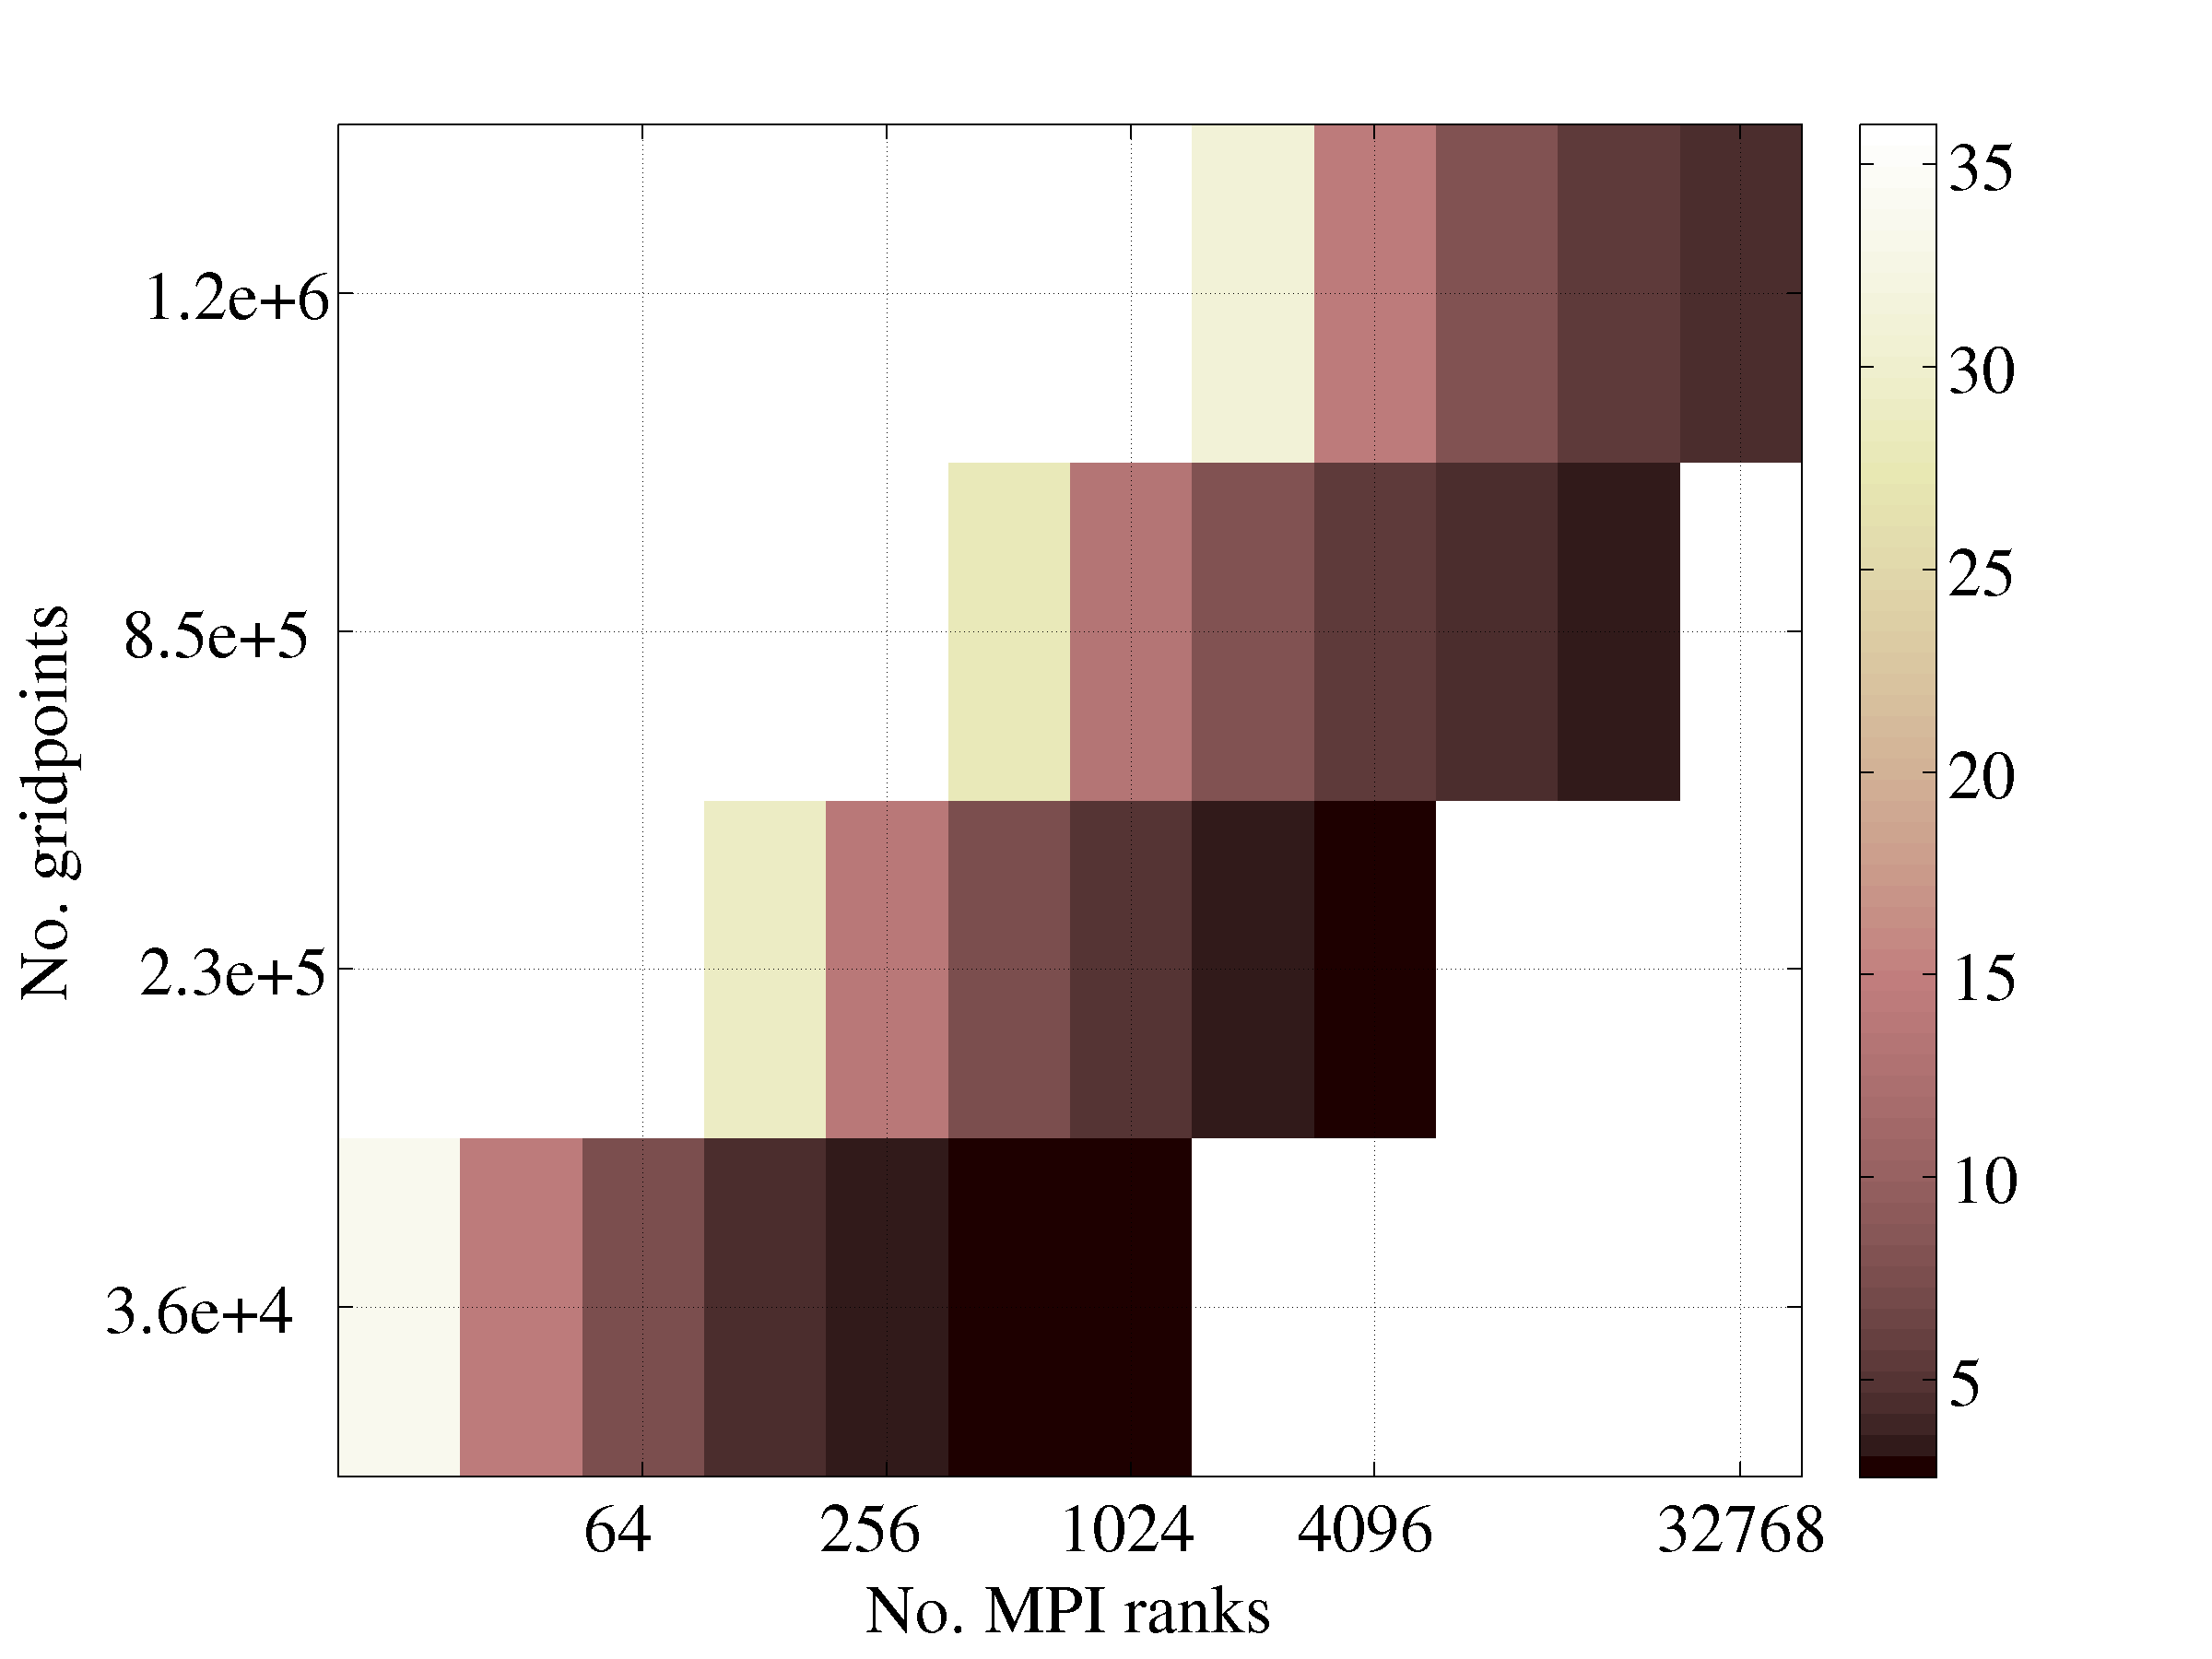
\includegraphics[width=\linewidth]{./figures/weak.png}
  \caption{Weak Scaling}
  \label{fig:weakscaling}
\end{figure}
\section{Conclusions}
%\end{document}  % This is where a 'short' article might terminate

%ACKNOWLEDGMENTS are optional
\section{Acknowledgments}

%
% The following two commands are all you need in the
% initial runs of your .tex file to
% produce the bibliography for the citations in your paper.
\bibliographystyle{abbrv}
\bibliography{easc2016}  % template.bib is the name of the Bibliography in this case
% You must have a proper ".bib" file
%  and remember to run:
% latex bibtex latex latex
% to resolve all references
%
% ACM needs 'a single self-contained file'!
%
%APPENDICES are optional
%\balancecolumns
\appendix
%Appendix A
\section{Appendix A}
\label{sec:plots}
% This next section command marks the start of
% Appendix B, and does not continue the present hierarchy

%\balancecolumns % GM June 2007
% That's all folks!
Test what is wrong
\end{document}

